%%
% 结论
% 结论是毕业论文的总结,是整篇论文的归宿,应精炼、准确、完整。结论应着重阐述自己的创造性成果及其在本研究领域中的意义、作用,还可进一步提出需要讨论的问题和建议。
% modifyer: 黄俊杰(huangjj27, 349373001dc@gmail.com)
% update date: 2017-04-13
%%

\chapter{总结与展望}


\section{本文工作的总结}

随着百度网盘的一家独大, 国内的在线文件分享服务格局从微博微盘, 华为Vdisk, 115网盘, 360云盘等多家服务提供商百花齐放, 竞争到如今基本只有百度和115能在较高收费的基础上提供高质量的在线文件存储、分享服务的格局。加之近日(2020年4月16日)有新闻报道百度网盘的限速策略破解软件PanDownload的作者被警方逮捕\footnote{突破百度网盘限速工具Pandownload作者被抓 非法获利30万余元: https://tech.sina.com.cn/roll/2020-04-15/doc-iircuyvh7984179.shtml}, 中文互联网的文件分享格局面临进一步的失控, 一旦百度公司宣布旗下的网盘服务停止运营或是大规模收费, 那对全中国互联网网民来说将是一个重大的利空。因此, 去中心化的文件存储、分享服务在笔者看来很有必要, 且势在必行。而BT作为成熟可靠的协议, 在过去的十数年间已有极为成功的网民间自发推广使用的历史。本文的工作目标便是将这一协议的价值重新发掘出来, 配以一个在线资源发布分享平台, 推广该协议在校内的使用。

在初期的开发选型过程中, 笔者及同好所在的团队经历过反复, 先选用了NexusPHP的衍生品天津大学北洋园TJUPT进行二次开发, 察觉到其巨大的二次开发难度后, 遂经过比较后转用UNIT3D, 随后开发步入正轨。

在数据的迁移过程中, 笔者通过使用修改适配后的数据库迁移脚本, 将原来NexusPHP上的数据表迁移至UNIT3D的数据表中, 并增加了必要的字段, 使用户能够较为无痛地从旧系统迁移至新系统。

在随后的功能完善实现中, 笔者剔除了不必要的标签系统功能, 完善实现了投票功能, 初步实现了鉴权操作日志记录功能。这些功能的调整为之后的上线内测运营打下了基础。

在一群行动力极强的同好的共同帮助下, 网站得以迅速上线运行。从初版基于天津大学北洋园TJUPT程序二次开发而来的网站于2019年12月19日上线, 到2020年2月26日网站转向使用UNIT3D-Community-Edition作为服务程序, 再到截至本文完成时刻\footnote{2020年4月22日}为止, 共发展了393位\footnote{根据用户ID}用户, 有850个资源。随着新学期的开始, 相信在强有力的校内推广下, 会逐渐发展出成熟、稳定的用户群。

笔者作为开发者参与了整个网站建设的全过程, 从初期站长突如其来地上线\footnote{2019年12月17日, 21weeks.icu上线内测}, 到站务、开发团队的招募与组建, 随后的开会讨论网站的技术转型, 再到NexusPHP转UNIT3D等的一系列工作, 无不饱含着每一位同好倾注的心血。

\section{本文工作的优缺点}

本文提出及实现实现到最终上线运营的资源分享平台, 具有如下优点:

\begin{enumerate}[label=\arabic*.,leftmargin=*]
\item UI美观。较其他大学流行的基于NexusPHP的PT网站有更加清晰的逻辑入口, 还包括响应式的自适应UI, 为手机用户浏览本站提供了一定的兼容性。

\item 稳定可靠。基于PHP语言的Laravel框架受益于其以来的PHP-FPM\footnote{https://php-fpm.org}运行时的所有优良特性, 包括进程式的请求响应管理, 将系统出错造成的损失局限在单独的进程之内, 相比如Node.js等因使用单线程处理事件循环\footnote{https://nodejs.org/en/docs/guides/event-loop-timers-and-nexttick/}(Event Loop)而需要更高成本的故障转移(Failover)的计算资源管理方式, 更不容易因为单点故障而导致网站可用性的下降(Degrade)。

\item 易于开发。Laravel框架的设计模式, 包括服务提供者(ServiceProvider), 事件机制, 以及完善自解释的MVC模型, 都为开发者提供了友好的开发体验。这为能够快速实现需求提供了难易度上的保证。

\item 已进入实际运营。与部分只停留在纸面上的论文不同, 作为工程类的论文, 本文的工作成果已经投入了实际的运营中\footnote{网站链接: https://21weeks.icu/}。随着用户群的稳步扩张, 加上即将开学\footnote{本文写于2020年4月19日}带来的新的一轮推广及用户招募, 本文的工作将会在更广阔的范围内显示其价值。

\item 持续完善中。本文所描述的资源分享平台在将来也会进行更多功能上的改进, 而非止步于本文列举的工作。在毕业后, 相信除了笔者以外, 会有更多志同道合的伙伴会加入到本项目的开发、运营、维护中来, 本文的工作也因此能得以持续完善。
\end{enumerate}


与此同时, 本文的工作也存在着不足, 包括:
\begin{enumerate}[label=\arabic*.,leftmargin=*]
\item NexusPHP的部分功能, 如页面小游戏功能和竞猜功能, 没能在这轮开发中得以迁移。因此新旧两版网站的用户体验并非无缝过渡。

\item 本文所做的工作之一的鉴权日志, 目前尚未实现前端的查询, 需要使用SQL终端或是SQL的管理用工具(如 MySQL Workbench\footnote{https://www.mysql.com/products/workbench}), 以及配合HTTP服务器本身的日志记录功能, 方可实现对鉴权日志的筛查。
\end{enumerate}

包括以上优缺点在内的特点既是本文笔者自豪的地方, 也是遗憾所在。

\section{展望}

文件分享, 作为计算机应用典型中的典型, 自互联网诞生以来, 就是所有网络用户需求之中最基础、也是最关键的一类。从最早的FTP协议, 到通过HTTP协议提供文件服务, 再到去中心化的BitTorrent, 以及今天衍生出的更彻底的去中心化协议IPFS\cite{DBLP:journals/corr/Benet14}, 不依赖Tracker、基于DHT\cite{andrewloewenstern2008bep0005}(Distributed Hashing Table)协议的BitTorrent扩展, 还有结合了HTTP和BT优点、基于WebRTC的Webtorrent, 技术一直在进步, 不论是网民自发推动的, 还是商业公司发起并推广甚至开源的。毫无疑问, 文件分享作为互联网的基础应用, 将长久地留存在所有互联网用户的使用习惯当中。

BitTorrent协议, 以及其标准中定义的Tracker服务器, 曾在很长一段时间内都是互联网文件分享的事实标准之一。至今仍有大量的BT用户于Tracker服务器活跃在世界各地, 秉持着分享精神这一人类的美好品质, 为有需要的人提供他们想要的资源。

本文所做的, 不过是站在BT协议这一巨人的肩膀之上, 在一所大学校园内, 建设了一个为校内用户使用的资源分享平台。与前人栽树的努力相比, 可以说是坐地乘凉般不足为道的微小工作。

然而笔者相信, 本文的工作必将有它巨大的价值。笔者坚信, 只要BT协议的使用习惯一旦形成, 将难以割舍, 用户群的分享精神将会得到激发。网盘固然好, 但资源的命脉始终被扼在一家以商业利益为终极目标的公司手中, 并不可靠。BT作为互联网分享精神的代表, 终将展现出其无限的潜能。

希冀于BT再一次在神州大地上开花结果!



% \chapter{总结与展望}
% \section{工作总结}
% \section{研究展望}
% \section{模板提供的命令}
% 冒号前面是命令,后面是显示的结果\\

% pozhehao(破折号):\pozhehao \sysuspace mybold\{com\}(加粗斜体):\mybold{com} \sysuspace  etoday:\etoday\sysuspace ctoday:\ctoday\sysuspace


% 用于equation环境的命令

% $norm :\norm{t}$

% $argmax:\argmax{x}{y}\sysuspace argmin:\argmin{x}{y}$

% $varmax:\varmax{x}{y}\sysuspace  varmin:\varmin{x}{y}$

% $fncmax:\fncmax{x}{y}\sysuspace  fncmin:\fncmin{x}{y}$

% $xxFnorm:\xxFnorm{x}\sysuspace xxFnormSqr:\xxFnormSqr{x}\sysuspace xxFprod:\xxFprod{x}{y}$

% $xxOpVec:\xxOpVec{x}\sysuspace xxLprod:\xxLprod{x}{y}\sysuspace xxLprodVec:\xxLprodVec{x}{y}\sysuspace xxTensor:\xxTensor{x}$

% $xxBracketY:\xxBracketY{x}\sysuspace xxBracketF:\xxBracketF{x}\sysuspace xxBracketH:\xxBracketH{x}$

% \begin{figure}
% 	\centering
% 	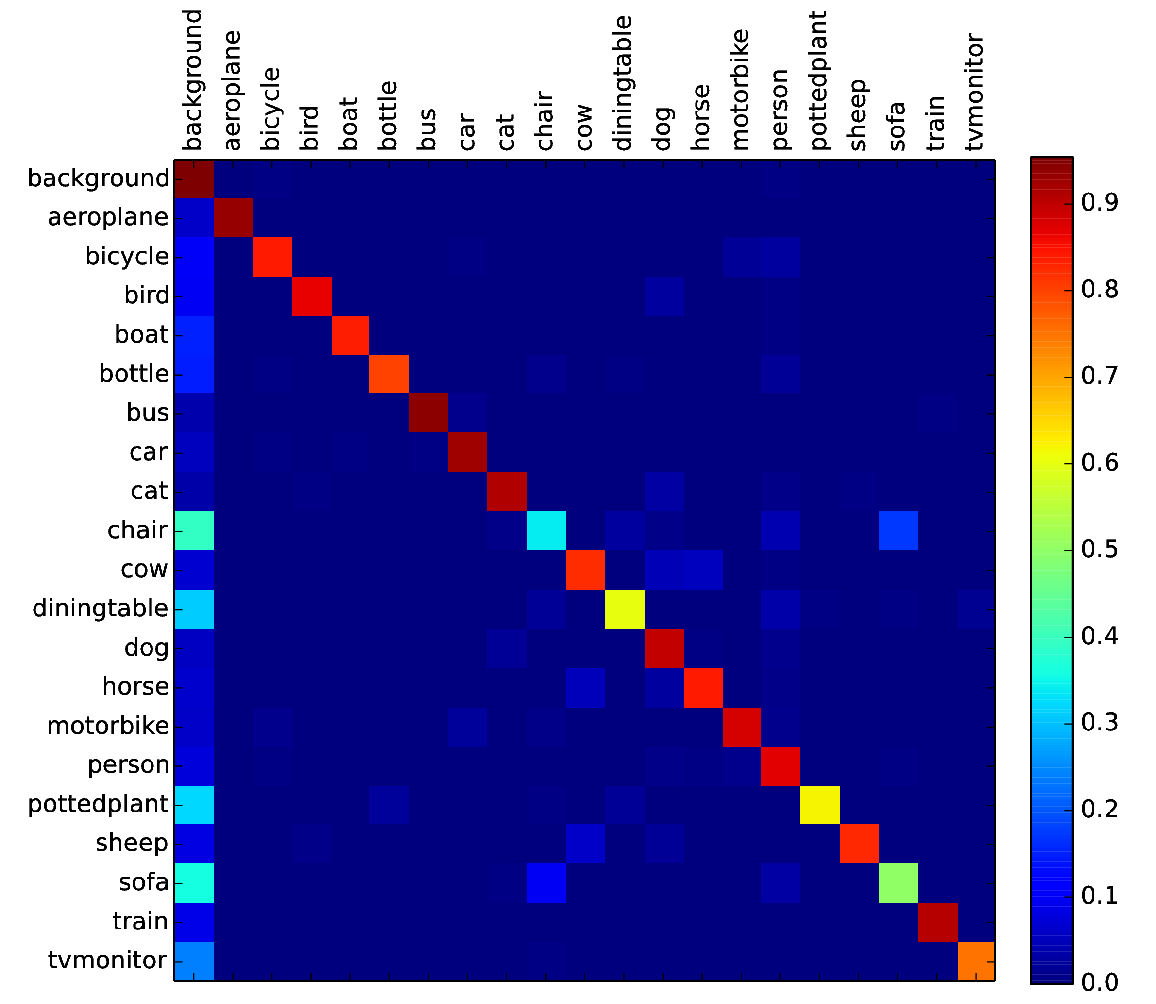
\includegraphics[width=0.5\textwidth]{image/result/confusion.pdf}
% 	\caption{镶嵌在文中的图像}
% 	\captionce[图注]{这是测试图注。}{A testing figure legend.}\label{fig:test}
% 	\label{fig:confusion}
% \end{figure}